\subsection{Design}
\subsubsection{Den statisk side af dasign}
Designdiagrammet i projektets anden iteration, blev opdateret med flere klasser og en tydelig lagdeling. En klar adskillelse af præsentations-, domæne- og persistenslaget er blevet illustreret og indeholder også subsystemernes klasser, med attributter og metoder. Det er valgt at getter og setter metoder ikke vises i diagrammet, da det ville gøre det meget større og sværere at overskue. (Se interne bilag figur \ref{fig:opklasse})\\
For at få et samlet overblik se interne bilag \ref{sec:diverse} figur \ref{fig:opklassemedlog} og figur \ref{fig:opklasse}\\ \\
\textbf{Præsentationslaget}
\begin{figure}[htb!]
  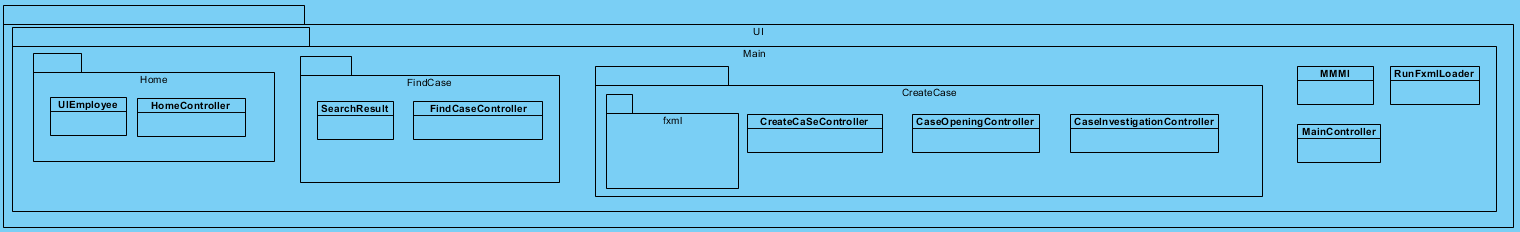
\includegraphics[width = \linewidth]{./PNG/design/UIopdateretKlassediagram.PNG} 
  \caption{Der blev valgt at undlade beskrivelsen af kontrollernes indhold og FXML-dokumenterne i subsystemet UI (Præsentationslaget), for at gøre diagrammet mere overskueligt. Præsentationslaget er blevet illustreret med pakker, som indeholder kontrollere og FXML-dokumenter for specifikke funktioner, samt klasserne som styrer systemets GUI.}
  \label{fig:2pre}
\end{figure}
\\\textbf{MainController – Præsentations controlleren}\\
Klassen ”MainController”, er systemets primære FXML-handler. Den blev lavet så det var muligt at skifte funktionalitet, på baggrund af et brugerinput, i samme root-node.\\\\
\textbf{RunFxmlLoader – Præsentationsmetoden}\\
Klassen ”RunFxmlLoader”, indeholder funktionaliteten som bruges til at skifte FXML-dokumenter. Den bliver arvet af ”MainController”, og implementere, som det eneste, metoden der bruges til at skifte ”pane”, i systemet.\\\\
\textbf{MMMI – Main Class}\\
Programmet køres gennem MMMI klassen, da det er programmets main class.\\\\
\textbf{CreateCase – Dokumentstyring og præsentation}\\
Subsystemet ”CreateCase”, blev designet til at begynde oprettelsen af nye sager i systemet og styre præsentationen af sagsdokumenter, samt brugerinteraktionen med disse. I slutningen af anden iteration var ”CreateCase”, pakket med kontrollerne ”CreateCaseController”, ”CaseOpeningController” og ”CaseInvestigationController”, samt FXML-pakken ”fxml”, som var pakket med de tilsvarende FXML-dokumenter.\\ 
Controlleren ”CreateCaseController”, blev designet til at styre bevægelsen mellem sagsdokumenter, samt at gemme brugerindtastet information fra disse dokumenter. Navngivningen kunne virke misvisende, i forhold til at controlleren bruges til at skifte mellem dokumenter, men peger på funktionaliteten bag gem funktionen. Når en given bruger benytter gem funktionen i en sag, sender controlleren de brugerindtastede informationer til domænelaget, for at få det registreret i systemdatabasen. \\
Hvis en sag gemmes for første gang i systemet, vil informationen som sendes gennem systemlagene, oprette en ny sag i databasen, som derefter modtager informationen. Controlleren er blevet navngivet efter denne proces, men har i sig selv kun at gøre med brugerinput og kommunikationen med domænelaget.\\
Controlleren ”CaseOpeningController”, er designet til at pakke informationerne indtastet i FXML- dokumentet ”caseOpeningNew”, og derefter sende det videre til ”CreateCaseController”, når en given bruger benytter gem funktionen.\\
Controlleren ”CaseInvestigationController”, har at gøre med informationen fra FXML-dokumentet ”caseInvestigation”. Controlleren er designet ligesom ”CaseOpeningController”, da de begge er designet til at håndtere information fra FXML-dokumenter, som er designet efter dokumenterne fra VUM. (Anon., 2019) \\
Designet af ”CreateCase”, var planlagt med fremtidig udvikling i tankerne, for at lave og implementere de dokumenter fra VUM, som mangler.\\ \\
\textbf{FindCase – Sagsrelateret søgning} \\
Subsystemet ”FindCase”, er designet til at håndtere et brugerinput, i form af en søgning, og præsentere information relateret til søgeordet. Subsystemet består af klassen ”SearchResult” og controlleren ”FindCaseController”, samt FXML-dokumentet ”findCase”.\\
Klassen ”SearchResult”, er en placeholder som fyldes med den data, der hentes på baggrund af en given brugers søgeord. Controlleren ”FindCaseController”, henter informationen som ”SearchResult”, består af og præsentere dem gennem FXML-dokumentet ”findCase”.\\\\
\textbf{Home – Systemets startside} \\
Subsystemet ”Home”, er designet til at håndtere systemets startside. Subsystemet består af klassen ”UIEmployee”, som er en placeholder klasse for medarbejderen der er logget ind i systemet og controlleren ”HomeController”, samt FXML-dokumentet ”home”.\\
Klassen ”UIEmployee”, er en placeholder klasse, som fyldes med information relateret til medarbejderen der er logget ind i systemet. Controllerklassen ”HomeController”, bruger informationen fra ”UIEmployee”, til at finde de relevante informationer som vedrør medarbejderen og præsentere dem gennem ”home”-dokumentet.\\\\
\textbf{Domænelaget}
\begin{figure}[htb!]
  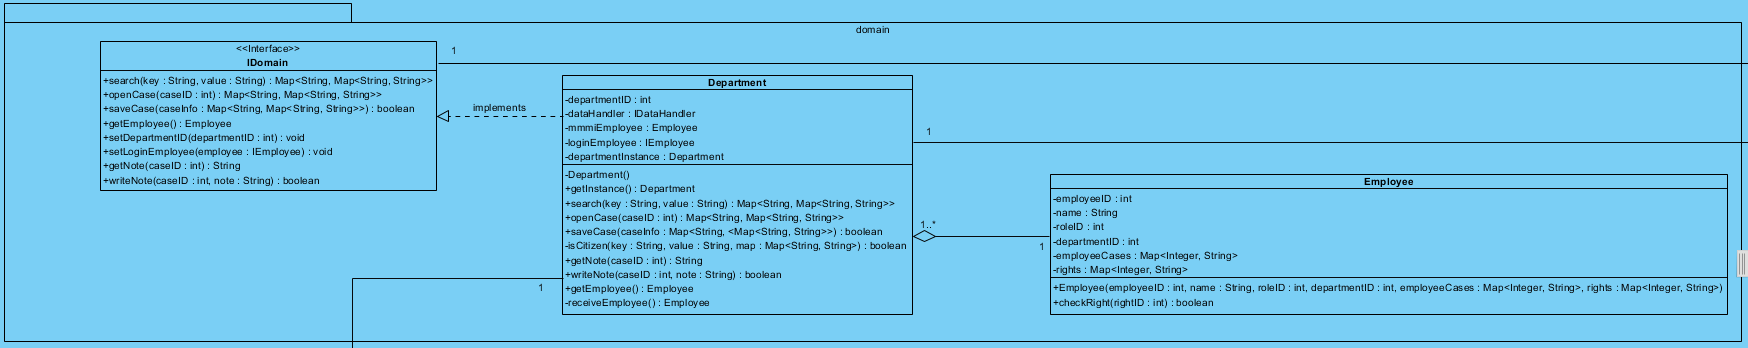
\includegraphics[width = \linewidth]{./PNG/design/domaeneOpdateretKlassediagram.PNG} 
  \caption{Domænelaget er blevet designet med to klasser, med attributter og metoder, og et interface.}
  \label{fig:2dom}
\end{figure}
\\\textbf{IDomain – Provided interface}\\
IDomain interfacet bruges til at vise præsentationslaget hvilke metoder der er tilgængelige i domænelaget, hvad de returnerer samt hvilke attributter der er nødvendige for at benytte metoderne. Interfacets metoder bliver implementeret i ”Department” klassen.\\\\
\textbf{Department – Facadeklasse}\\
Klassen ”Department” har en private constructor “Department()”, attributterne ”departmentID”, ”dataHandler”, ”mmmiEmployee”, ”loginEmployee” og ”departmentInstance”, samt metoderne ”getInstance()”, ”search(…)”, ”openCase(…)”, ”saveCase(…)”, ”isCitizen(…)”, ”getNote(…)”, ”writeNote(…)”, “getEmployee()” og “receiveEmployee()”.\\
For at imødekomme projektets underspørgsmål ”Hvordan sikres det at aktøren kun har adgang til det aktøren har brug for?” og dataafgrænsningen fra sagsudredning i semestercasen, er der blevet lagt stor vægt på attributten “departmentID”. \\
Dette ID tildeles via en setter metode, ”setDepartmentID(…)”, når en medarbejder logger ind i systemet. Singleton designpattern blev valgt, da der er nødvendigt at være sikre på at det er det samme ”Department”-objekt der arbejdes med gennem hele systemet.\\\\
\textbf{Employee – Dataklasse, repræsenterer den medarbejder der er logget ind}\\
Klassen ”Employee” er designet til at håndtere tjek af rettigheder i forhold til forskellige medarbejderroller. Når en bruger logger ind i systemet, sendes der en employeeID til ”Department” som kalder persistenslaget for at få data om medarbejderen for at oprette en instans af Employee.\\
Dette gøres for at det kan være muligt at der er styr på hvem der er logget ind, samt have mulighed for at tjekke rettighederne som medarbejderen har gennem metoden ”checkRight(…)”.\\ \\
\textbf{Persistenslaget}
\begin{figure}[htb!]
  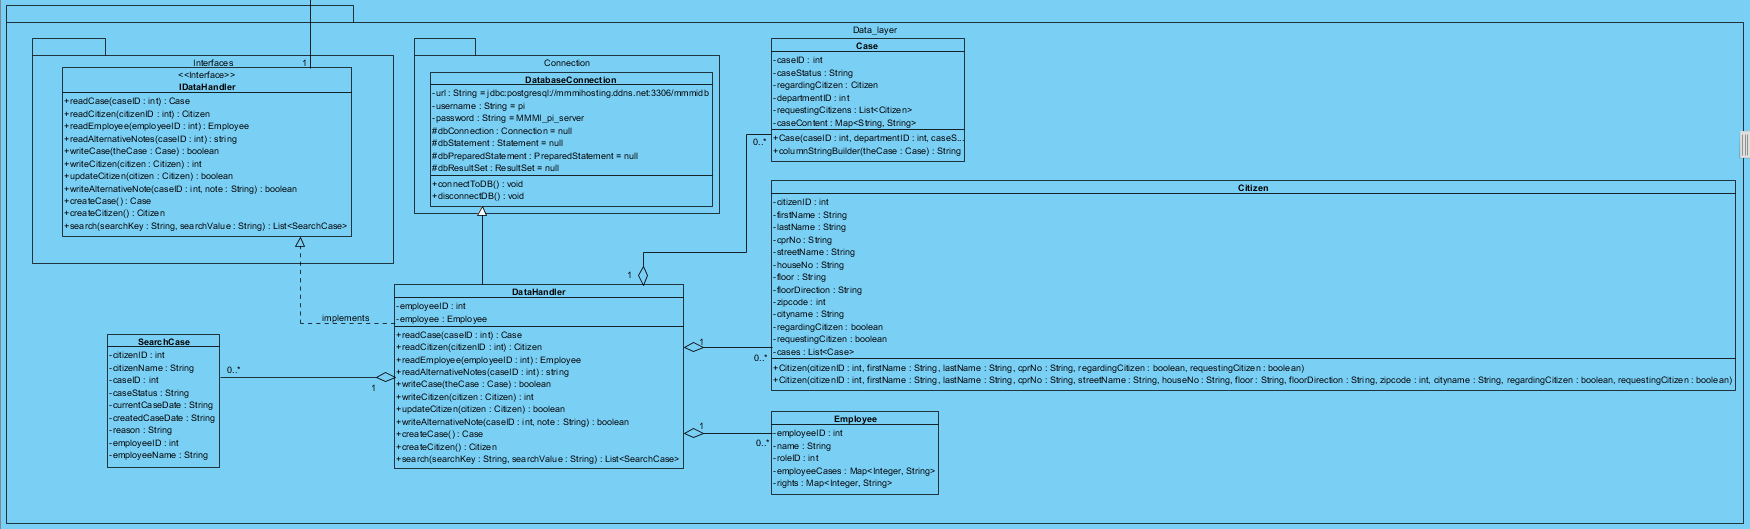
\includegraphics[width = \linewidth]{./PNG/design/datalagKlassediagram.PNG} 
  \caption{Persistenslaget er blevet designet med seks klasser og et interface.}
  \label{fig:2dataklassediagram}
\end{figure}
\\ 
\textbf{IDataHandler – Provided interface} \\
Interfacet ”IDataHandler”, bruges til at tillade og etablere kontakten mellem domænelaget og persistenslaget. Metoderne som interfacet består af implementeres i ”DataHandler” klassen og kaldes i domænelaget, når databasen skal kontaktes.\\
\textbf{DataHandler – Facadeklasse}\\
Klassen ”DataHandler”, er blevet designet til at håndtere dataforespørgsler sendt fra domænelaget og behandle dem som ønsket i systemets database. Klassen implementerer ”IDataHandler” interfacet og metoderne der følger med, som specificeres så data bliver hentet og/eller gemt, når de bliver kaldt fra domænet.\\
Når der skal hentes data fra databasen, er metoderne ”readCase(…)”, ”readCitizen(...)”, ”readEmployee(…)”, ”readAlternativeNotes(…)” og ”search(…)”, blevet designet for at kunne tilgå specifikke koloner, så den relevante information kan blive hentet. \\
Designet er lavet så at, når der skal gemmes data i databasen, benyttes metoderne ”writeCase(…)”, ”writeCitizen(…)”, ”updateCitizen(…)” og ”writeAlternaticeNote(…)”. Metodekaldet der skal bruges, afhænger af hvilken information der ønskes gemt. \\
Klassens associationer består primært af aggregeringer, med multipliciteten one-to-zero-or-many. ”DataHandler” er forbundet med aggregeringer til klasserne ”SearchCase”, ”Case”, ”Citizen” og ”Employee”. \\\\
\textbf{SearchCase – Placeholder til data fra “search(…)”}\\
Klassen ”SearchCase” indeholder udelukkende attributterne ”citizenID”, ”citizenName”, ”caseID”, ”caseStatus”, ”currentCaseDate”, ”createdDateCase”, “reason”, “employeeID”, “employeeName”.  Klassen bruges når der søges i databasen med metoden ”search(…)”, til at indeholde de data der er relevant at vise brugeren, i forhold til at kunne vælge den rigtige sag at åbne.\\\\
\textbf{Employee – Dataklasse, repræsenterer en medarbejder og alle dennes tilknyttede sager i afdeling}\\
Klassen ”Employee” indeholder udelukkende attributterne ”employeeID”, ”name”, ”roleID”,\\ ”employeeCases” og ”rights”. \\\\
\textbf{Case – Dataklasse, repræsenterer en sag}\\
Klassen ”Case” indeholder attributterne “caseID”, “caseStatus”, “regardingCitizen”, “departmentID” som alle skal bruges for at oprette en ny sag i tabellen ”case” i databasen. Yderligere er der en attribut ”requestingCitizen”, som skal bruges for at forbinde en sag med en eventuel henvendende borger, samt en attribut ”caseContent”, som indeholder alle oplysninger som en sagsbehandler kan indtaste. \\
Der er også en constructor som sætter alle attributterne, samt en metode der bruges til at konstruere den query, som sørger for at ”caseContent”, bliver gemt i databasen.\\ \\
\textbf{Citizen – Dataklasse, repræsenterer en borger og alle dennes oprettede sager i afdeling}\\
Klassen ”Citizen” indeholder attributterne ”citizenID”, ”firstName”, ”lastName”, ”cprNo”, ”streetName”, ”houseNo”, ”floor”, ”floorDirection”, ”regardingCitizen”, ”requestingCitizen”, ”Cases”. Den har 2 constructore, en som har de primære attributter der skal bruges for at oprette en Citizen i database, og en anden som har alle attributter.\\\\
\textbf{DataConnection – Håndtering af forbindelse til database}\\
Klassen ”DataConnection” blev implementeret for at vi kunne have de nødvendige informationer til at forbinde med databasen placeret et sted som kunne genbruges i andre moduler. \\
\subsubsection{Den dynamisk side af design}
\begin{figure}[htb!]
  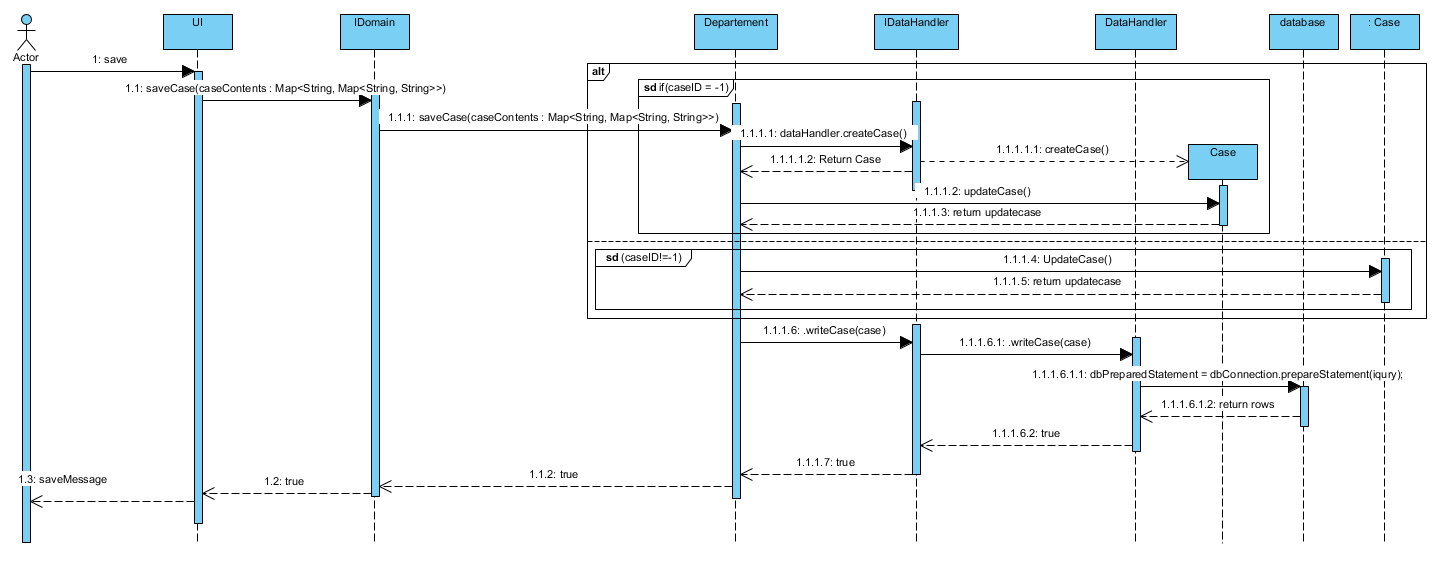
\includegraphics[width = \linewidth]{./PNG/design/odyn.PNG} 
  \caption{Sekvensdiagram for savecase}
  \label{fig:2savecase}
\end{figure}
\textbf{saveCase}
Når en aktør har udfyldt vilkårlige felter i sagsdokumenterne, kan denne data gemmes i databasen. \\
Når aktøren benytter ”1.save”, gemmes alt data der er indtastet i et contentsMap af typen ”Map\textless String, Map\textless String, String\textgreater \textgreater ”. Der benyttes et Map af Maps for at minimere koblingen. \\
Når contentsMap gemmes, benyttes metoden ”saveCase(…)” der sender den data igennem interfacet ”IDomain” ned til ”Department” facaden. Denne bliver pakket ud via metoden saveCase(…), i klassen Department, og tjekker på ”caseID” om det er lig med -1. Hvis dette er tilfældet, sender den Map ned videre igennem IDataHandler interfacet og ned til DataHandler. SaveCase(…) metoden i Datahandleren tjekker om der er en ny Case på caseID, hvis denne er -1, benyttes createCase() metoden der opretter et ”Case” objekt.\\
Hvis en Case allerede findes i Databasen, bliver updateCase() metoden kaldt, som opdatere ”Case” objektet og returner det opdaterede Case objekt. \\
Metoden som skriver i tilfældet af et eksisterende Case objekt eller et nyt Case objekt (1.1.1.6), benytter writeCase(…) metoden(1.1.1.6.1), som modtager et Case objekt og herefter skriver det ind i databasen ved at benytte en Prepared Statement. 
Hvis alle trin udføres succesfuldt, kvitteres der ”true” tilbage til aktøren. 
\begin{figure}[htb!]
  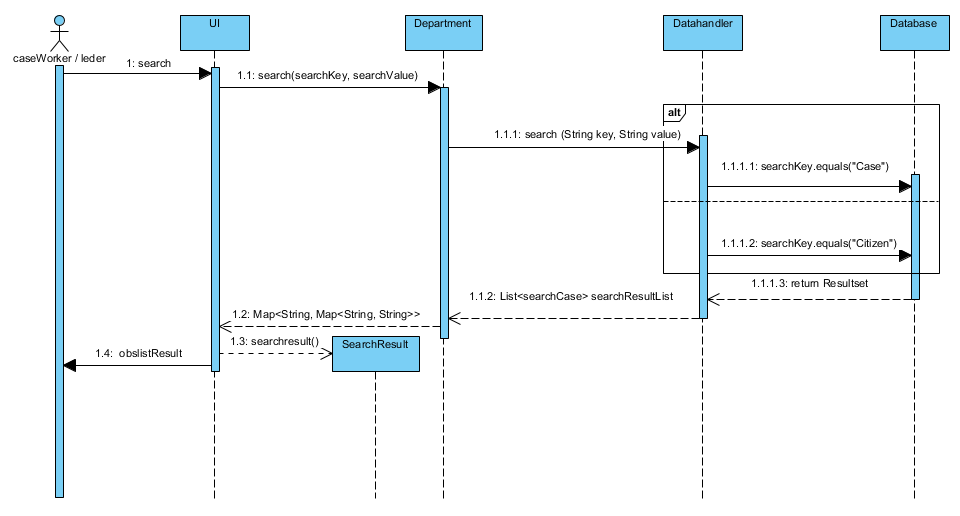
\includegraphics[scale = 0.55]{./PNG/design/seksearch.PNG} 
  \caption{Sekvensdiagram for search. Se interne bilag figur \ref{fig:seksearch}}
  \label{fig:2savecase}
\end{figure}
\\\textbf{Search}\\
1.	Personalet benytter søgefunktionen i systemet.\\
Denne bruges for at finde en eller flere sager på en given borger. \\
1.1.	En searchKey er blevet valgt i præsentationslaget og et searchValue er blevet\\ indtastet. Disse informationer sendes via Department metoden ”search(…)” , til domænelaget. \\
Den valgte ”searchKey” bruges til at vælge om der søges efter en specifik sag, eller sager der er relateret til en person. ”searchValue” bruges til at identificere de relevante informationer.\\
1.1.1.	Den valgte ”searchKey” bliver sendt videre som en ”String key” og searchValue bliver sendt videre som ”String value” i datahandler metoden search(…). \\
”StringKey” bestemmer hvilke SQL statement der skal bruges i persistenselaget. ”String value” er de værdier der skal matches i databasen. \\
1.1.1.1.	Her bliver der undersøgt om den ”String key” der er blevet modtaget, har værdien ”Case”\\
1.1.1.2.	 Her bliver der undersøgt om den ”String key” der er blevet modtaget, har værdien ”Citizen”. \\
Afhængigt af værdien, ”Case” eller ”Citizen”, vil en SQL kode blive kørt og hente informationer relateret til ”String value” fra 1.1.1.\\
1.1.1.3.	Databasen returner et ”ResultSet” med de værdier den har fundet. \\
Der bliver kun returneret data fra databasen, hvis ”departmentid” er i overensstemmelse med det der står i databasen. \\
1.1.2.	Data bliver pakket ind i  ”SearchCase” objekter og bliver gemt i en ”List\textless SearchCase\textgreater searchResultList” liste.\\
Denne liste sendes til domænelaget for at datapakken kan bearbejdes derfra. \\
1.2.	De modtagede ”SearchCase” objekter bliver læst og skrevet ind i ”searchResultMap”. Disse Maps bliver skrevet ind i HashMap ”searchResultList”.\\
Der bliver sendt et Map af Maps fordi ”SearchCase” objekterne ikke kan blive sendt videre til præsentationslaget. Vi minimerer kobling mellem lagende ved at skifte en liste af ”SearchCase” objekter  og udskifter dem med Map af Maps.\\
1.3.	Det modtagede ”Map\textless String, Map\textless String, String\textgreater \textgreater ” pakkes ud og opretter ”SearchResult” objekter af de inderste Maps. \\
1.4.	Alle ”SearchResult” objekter bliver tilføjet til en ”ObservableList\textless SearchResult\textgreater ”. \\
Der oprettes ”SearchResult” objekter for at kunne præsentere de modtagede informationer. Disse informationer tilføjes derefter til en ”ObservableList\textless SearchResult\textgreater ” liste for at ”TableView” kan præsentere de fundne informationer til brugeren. \\